\begin{frame}[fragile]
\begin{layout-full}
\begin{center}
\begin{onlyenv}<1->
\begin{tikzexample}
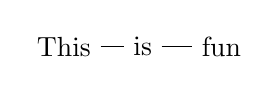
\begin{tikzpicture}
   \foreach[count=\i] \name in {
      This, is, fun
   } {
      \node (\i) at (\i,.75) {\name};
   }
   \draw (1) -- (2) -- (3);
\end{tikzpicture}
\end{tikzexample}
\end{onlyenv}
\end{center}
\end{layout-full}
% foreach is not limited to tikzpictures...
\end{frame}

{%
\def\ExampleBoundingBox{(-.75,-2) rectangle (2.6,1.6)}
\begin{frame}[fragile]
\begin{layout-full}
\begin{center}
\begin{onlyenv}<2->
\begin{tikzexample}
\begin{tikzpicture}
   \pingu[heart,
      eyes shiny,
      feet sit,
      tie=blue
   ]
\end{tikzpicture}
\end{tikzexample}
\end{onlyenv}
\end{center}
\end{layout-full}
\begin{tikzpicture}[@O]
   \only<2->{\node[above right=2mm,gray,font=\scriptsize] at(current page.south west) {\href{https://github.com/EagleoutIce/tikzpingus}{github.com/EagleoutIce/tikzpingus}};}
\end{tikzpicture}
% TODO: penguins
\end{frame}
}
{%
\def\ExampleBoundingBox{(-.75,-2) rectangle (2.6,1.6)}
\begin{frame}[fragile]
\begin{lrbox}\CodeBox
\begin{minipage}{.925\linewidth}
\begin{minted}{latex}
\begin{tikzpicture}[overlay, remember picture]
   \node[below left] at (current page.north east)
      {Hello World!};
\end{tikzpicture}
\end{minted}
\end{minipage}
\end{lrbox}
\begin{focus}
   \usebox\CodeBox\vspace*{4em}\\*
   \onslide<3->{\blatex{\\usepackage\{tcolorbox\}} \qquad \blatex{\\usepackage\{pgfplots\}}}\medskip\\
   \onslide<3->{\blatex{\\usepackage\{forest\}}}
\end{focus}
\begin{onlyenv}<2->
\begin{tikzpicture}[overlay,remember picture]
   \node[below left] at(current page.north east) {Hello World!};
\end{tikzpicture}
\end{onlyenv}
% tikz absolute placement
% refernce forest, tcolorbox and pgfplots
\end{frame}
}

\Learning{Ti\textit{k}Z Is Great for Smaller Graphics!}{And for more advanced stuff as well, but let's stick to the basics\ldots}
